\section{Gorder}
Gorder\cite{wei2016speedup} は演算時のアクセス局所性に着目し,有向グラフ上で任意の2ノード u, v 間に \textit{neighbor relationship} と \textit{sibling relationship} を定義する.
そして,これらの関係に基づいてノード u, ノード v の近接度合いをスコア化する.
neighbor relationship に基づくスコアでは,ノード u,ノード v が双方向にエッジを張っている場合+2,
ノード u,ノード v の一方から他方へエッジが張られている場合+1,ノード u,ノード v 間にエッジが張られていない場合+0 となる.
また,sibling relationship に基づくスコアでは,ノード u,ノード v が共通のノード x からエッジを張られている場合+1 となり,
ノード x の数に応じてスコアが加算されていく.
neighbor relationship を図\ref{neighbor} に,sibling relationship を図\ref{sibling} に示す. 
\begin{figure}[t]
  \begin{tabular}{cc}
    \begin{minipage}[t]{0.45\hsize}
      \centering
      %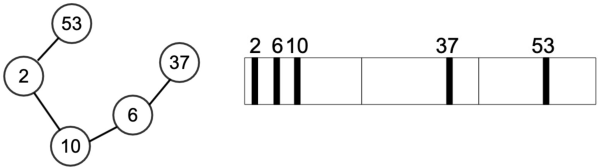
\includegraphics[keepaspectratio, scale=0.50]{./figure/id_not_consecutive.pdf}
      %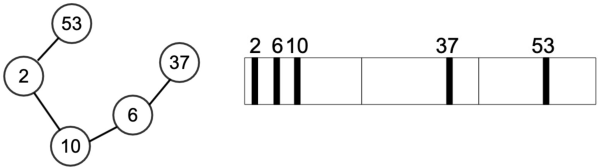
\includegraphics[keepaspectratio, width=7cm]{./figure/id_not_consecutive.pdf}
      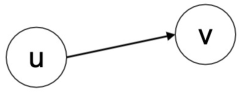
\includegraphics[width=6.5cm]{./figure/neighbor.pdf}
      %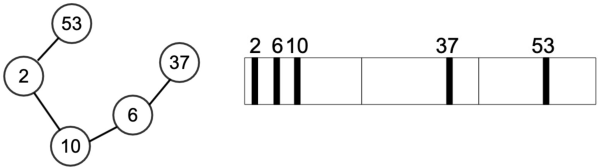
\includegraphics[scale=0.50]{./figure/id_not_consecutive.pdf}
      \caption{neighbor relationship}
      \label{neighbor}
    \end{minipage} &
    \begin{minipage}[t]{0.45\hsize}
      \centering
      %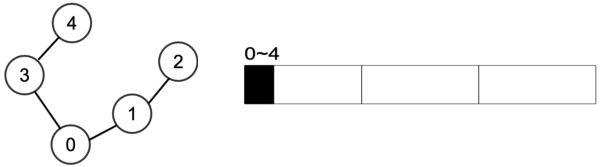
\includegraphics[keepaspectratio, scale=0.50]{./figure/id_consecutive.pdf}
      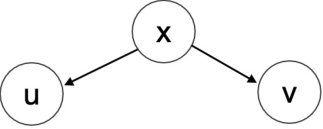
\includegraphics[width=7cm]{./figure/sibling.pdf}
      %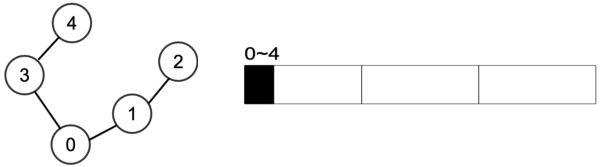
\includegraphics[scale=0.50]{./figure/id_consecutive.pdf}
      \caption{sibling relationship}
      \label{sibling}
    \end{minipage}
  \end{tabular}
\end{figure}
ここで,neighbor relationship に基づくスコアを $S_{n}(u,v)$,sibling relationship に基づくスコアを $S_{s}(u,v)$としたとき,
ノード u,ノード v のスコア $S(u,v)$ は(\ref{gorder_score})式で定義される.
\begin{equation}
  S(u,v) = S_{n}(u,v) + S_{s}(u,v) \label{gorder_score}
\end{equation}
そして,ノード u,ノード v の ID がそれぞれ $\phi(u)$,$\phi(v)$に変換される時,
(\ref{gorder})式で定義する $F(\phi)$ を最大化する ID 配置 $\phi$ に基づいて再配置を実行する.
\begin{equation}
  F(\phi) = \sum_{0<\phi(v)-\phi(u)\leq3}^{} S(u,v) \label{gorder}
\end{equation}
なお,図\ref{reordering_intro} は Gorder の例を示しており,(\ref{gorder})式で定義される$F(\phi)$ を最大化するように ID が再配置されている.
Gorder はグラフ演算速度の向上率という観点では最良の ID 再配置手法だが,前処理の時間コストが大きすぎるため非実用的と指摘されている\cite{balaji2018graph, faldu2019closer}.
\section{Degree Sorting}
DegreeSorting は次数による局所性のみに着目し,高次数ノードから昇順の ID を再配置していく.
図\ref{Original} で示す 12 ノードを Degree Sorting で再配置する場合の例を図\ref{degree_sorting} で示す.
なお,図\ref{Original} では,平均次数 20 を越えるノードは薄い赤色,平均次数の 2 倍である 次数 40 を越えるノードは濃い赤色で示されている.
次数に基づくソードにより,ID が近いノードは同程度の次数であることが保証されるため,次数による局所性を十分に考慮することができる.
しかし,\cite{balaji2018graph, faldu2019closer} などで元の ID が近いノードはグラフ上で近接していることが明らかになっている.
そのため,次数によるソートでグラフの近接構造を表す情報が失われてしまい,近接構造による局所性を考慮することが不可能となる.
\begin{figure}[t]
  \centering
  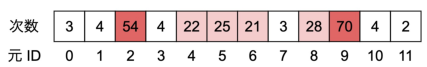
\includegraphics[width=\linewidth]{./figure/original.pdf}
  \caption{再配置対象のノード ID と次数情報}
  \label{Original}
\end{figure}
\begin{figure}[t]
  \centering
  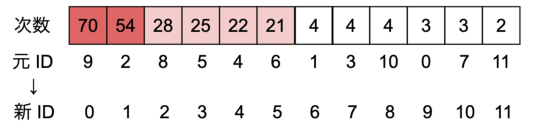
\includegraphics[width=\linewidth]{./figure/degree_sorting.pdf}
  \caption{Degree Sorting による再配置の例}
  \label{degree_sorting}
\end{figure}
\section{Hub Sorting}
Hub Sorting \cite{zhang2017making} は,Degree Sorting と同様に次数による局所性に着目しているが,高次数ノードのみ次数に基づくソートを実行し ID を再配置している.
これにより,低次数ノードでは近接構造による局所性を維持しつつ,アクセスが集中する高次数ノードでは次数による局所性を考慮している.
Hub Sorting では,平均次数以上の次数を持つノードを高次数ノードとみなしているが,
実世界グラフおいて平均次数以上のノードに接続しているエッジは全体の 80 - 90 \% を占める\cite{faldu2019closer}.
そのため,高次数ノードにおいても近接構造による局所性を考慮した ID 再配置を実行する必要があるが,
Hub Sorting による再配置では高次数ノードでの近接構造による局所性を考慮できていないという問題点が存在する.
図\ref{hubclustering} で Hub Sorting による再配置の例を示すが,平均次数 20 を越える高次数ノード内で元の ID の順序が保たれていないことが確認できる.
\begin{figure}[t]
  \centering
  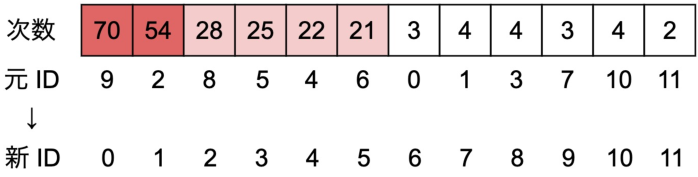
\includegraphics[width=\linewidth]{./figure/hubsorting.pdf}
  \caption{Hub Sorting による再配置の例}
  \label{hubsorting}
\end{figure}
\section{Hub Clustering}
Hub Clustering \cite{balaji2018graph} は,Hub Sorting における問題点に着目し,高次数ノード内でソートを行わずに元の ID 順を保った再配置を行うことで
高次数ノードでの近接構造による局所性を考慮している.
しかし,実世界グラフはスケールフリー性を持つため,平均次数以上のノード内でも次数分布には大きな偏りが発生する.
そのため,Hub Clustering では,高次数ノード内での次数分布の偏りを考慮した ID 再配置が行えていないという問題点が存在する.
図\ref{hubclustering} で Hub Clustering による再配置の例を示す.
Hub Sorting と比較して高次数ノード内でも元の ID 順が保たれているが,次数 54 と次数 70 のノードに連続した ID を再配置できていないことが確認できる.
\begin{figure}[t]
  \centering
  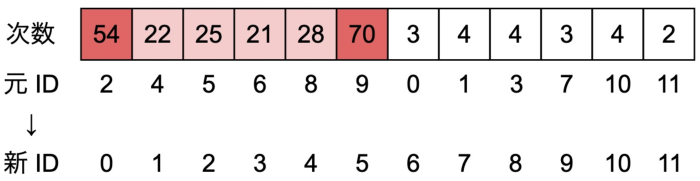
\includegraphics[width=\linewidth]{./figure/hubclustering.pdf}
  \caption{Hub Clustering による再配置の例}
  \label{hubclustering}
\end{figure}
\section{Degree Based Grouping (DBG)}
\label{dbg}
Hub Sorting や Hub Clustering で問題が生じる主要な要因は,平均次数というただ1つの境界値に基づき高次数ノードと低次数ノードを二分しているからである.
そこで,DBG \cite{faldu2019closer}はグラフの平均次数$\mathbb{A}$に基づき,[0,$\mathbb{A}$/2),[$\mathbb{A}$/2,$\mathbb{A}$),[$\mathbb{A}$,2$\mathbb{A}$),[2$\mathbb{A}$,4$\mathbb{A}$),
[4$\mathbb{A}$,8$\mathbb{A}$),[8$\mathbb{A}$,16$\mathbb{A}$),[16$\mathbb{A}$,32$\mathbb{A}$),[32$\mathbb{A}$,$\infty$)
と 次数の範囲が異なる 8 グループを定義し,各ノードを次数でグループ分けする.
HubSorting や HubClustering は,[0,$\mathbb{A}$),[$\mathbb{A}$,$\infty$) の 2 グループしか定義されていないため,
高次数ノード内での次数分布の偏りに対応できていないが,DBG では 8 グループ定義することで次数分布の偏りに対応している.
そして,高次数のグループから元の ID 順を保って昇順の連続した ID を再配置することで次数による局所性と近接構造による局所性の双方を考慮している.
DBG による再配置の例を図\ref{dbg} で示す.
\begin{figure}[t]
  \centering
  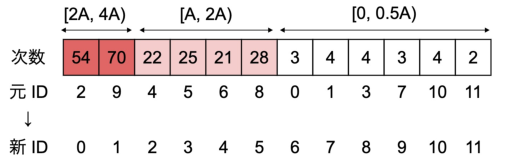
\includegraphics[width=\linewidth]{./figure/dbg.pdf}
  \caption{DBG による再配置の例}
  \label{sec:dbg}
\end{figure}
\section{まとめ}
本章では,既存の代表的な ID 再配置手法として,Gorder,Degree Sorting,Hub Sorting,Hub Clustering を紹介した.
また,本章で紹介した手法以外にも,Rabbit Order \cite{arai2016rabbit},ReCall \cite{lakhotia2017recall},Slash Burn \cite{kang2011beyond},
METIS \cite{karypis1998multilevelk} などの手法が提案されている.
しかし,既存手法はグラフの全体構造が把握可能という前提のもと議論されている.
そのため,グラフ取得の完了まで全グラフが手元にない状況へ既存手法を適用することは困難であり,グラフを取得しながら ID を再配置するという手法は存在しない.